\documentclass[tikz]{standalone}
\usepackage[utf8]{inputenc}
\usepackage[T1]{fontenc}
\usepackage[forget]{qrcode}
\usepackage{fontawesome5}
\newlength{\qrwd}
\setlength{\qrwd}{25mm}
\begin{document}
\begin{tikzpicture}
\node[%
%   draw      = white,%
%   fill      = white,%
  anchor    = south west,%
  inner sep = 0,%
] at (0, 0) (QRCode) {%
  \qrcode[height = \qrwd, level = M]{https://www.utfpr.edu.br/campus/pontagrossa}%
};
\begin{scope}[x = {(QRCode.south east)}, y = {(QRCode.north west)}]
\node[%
  circle,%
  fill      = blue!50!gray,%
  text      = white,%
  anchor    = center,%
  inner sep = 0,%
] at (0.5, 0.5) (Logo) {%
  {\fontsize{0.2\qrwd}{0.2\qrwd}\selectfont\faLink}%
};
\end{scope}
\end{tikzpicture}
\end{document}
